\begin{ujnbody}
    \chapter{基础功能测试}
    \section{文字与段落}
    这是文字。

    这是段落。这是段落。这是段落。这是段落。这是段落。这是段落。这是段落。这是段落。这是段落。这是段落。这是段落。这是段落。这是段落。这是段落。这是段落。这是段落。这是段落。这是段落。
    \subsection{文字与段落}
    这是文字。

    这是段落。这是段落。这是段落。这是段落。这是段落。这是段落。这是段落。这是段落。这是段落。这是段落。这是段落。这是段落。这是段落。这是段落。这是段落。这是段落。这是段落。这是段落。
    \section{文字与段落}
    这是文字。

    这是段落。这是段落。这是段落。这是段落。这是段落。这是段落。这是段落。这是段落。这是段落。这是段落。这是段落。这是段落。这是段落。这是段落。这是段落。这是段落。这是段落。这是段落。
    \section{文字与段落}
    这是文字。

    这是段落。这是段落。这是段落。这是段落。这是段落。这是段落。这是段落。这是段落。这是段落。这是段落。这是段落。这是段落。这是段落。这是段落。这是段落。这是段落。这是段落。这是段落。
    \section{文字与段落}
    这是文字。

    这是段落。这是段落。这是段落。这是段落。这是段落。这是段落。这是段落。这是段落。这是段落。这是段落。这是段落。这是段落。这是段落。这是段落。这是段落。这是段落。这是段落。这是段落。
    \section{图表}

    \subsection{图片}

    \begin{figure}[htbp]
        \centering
        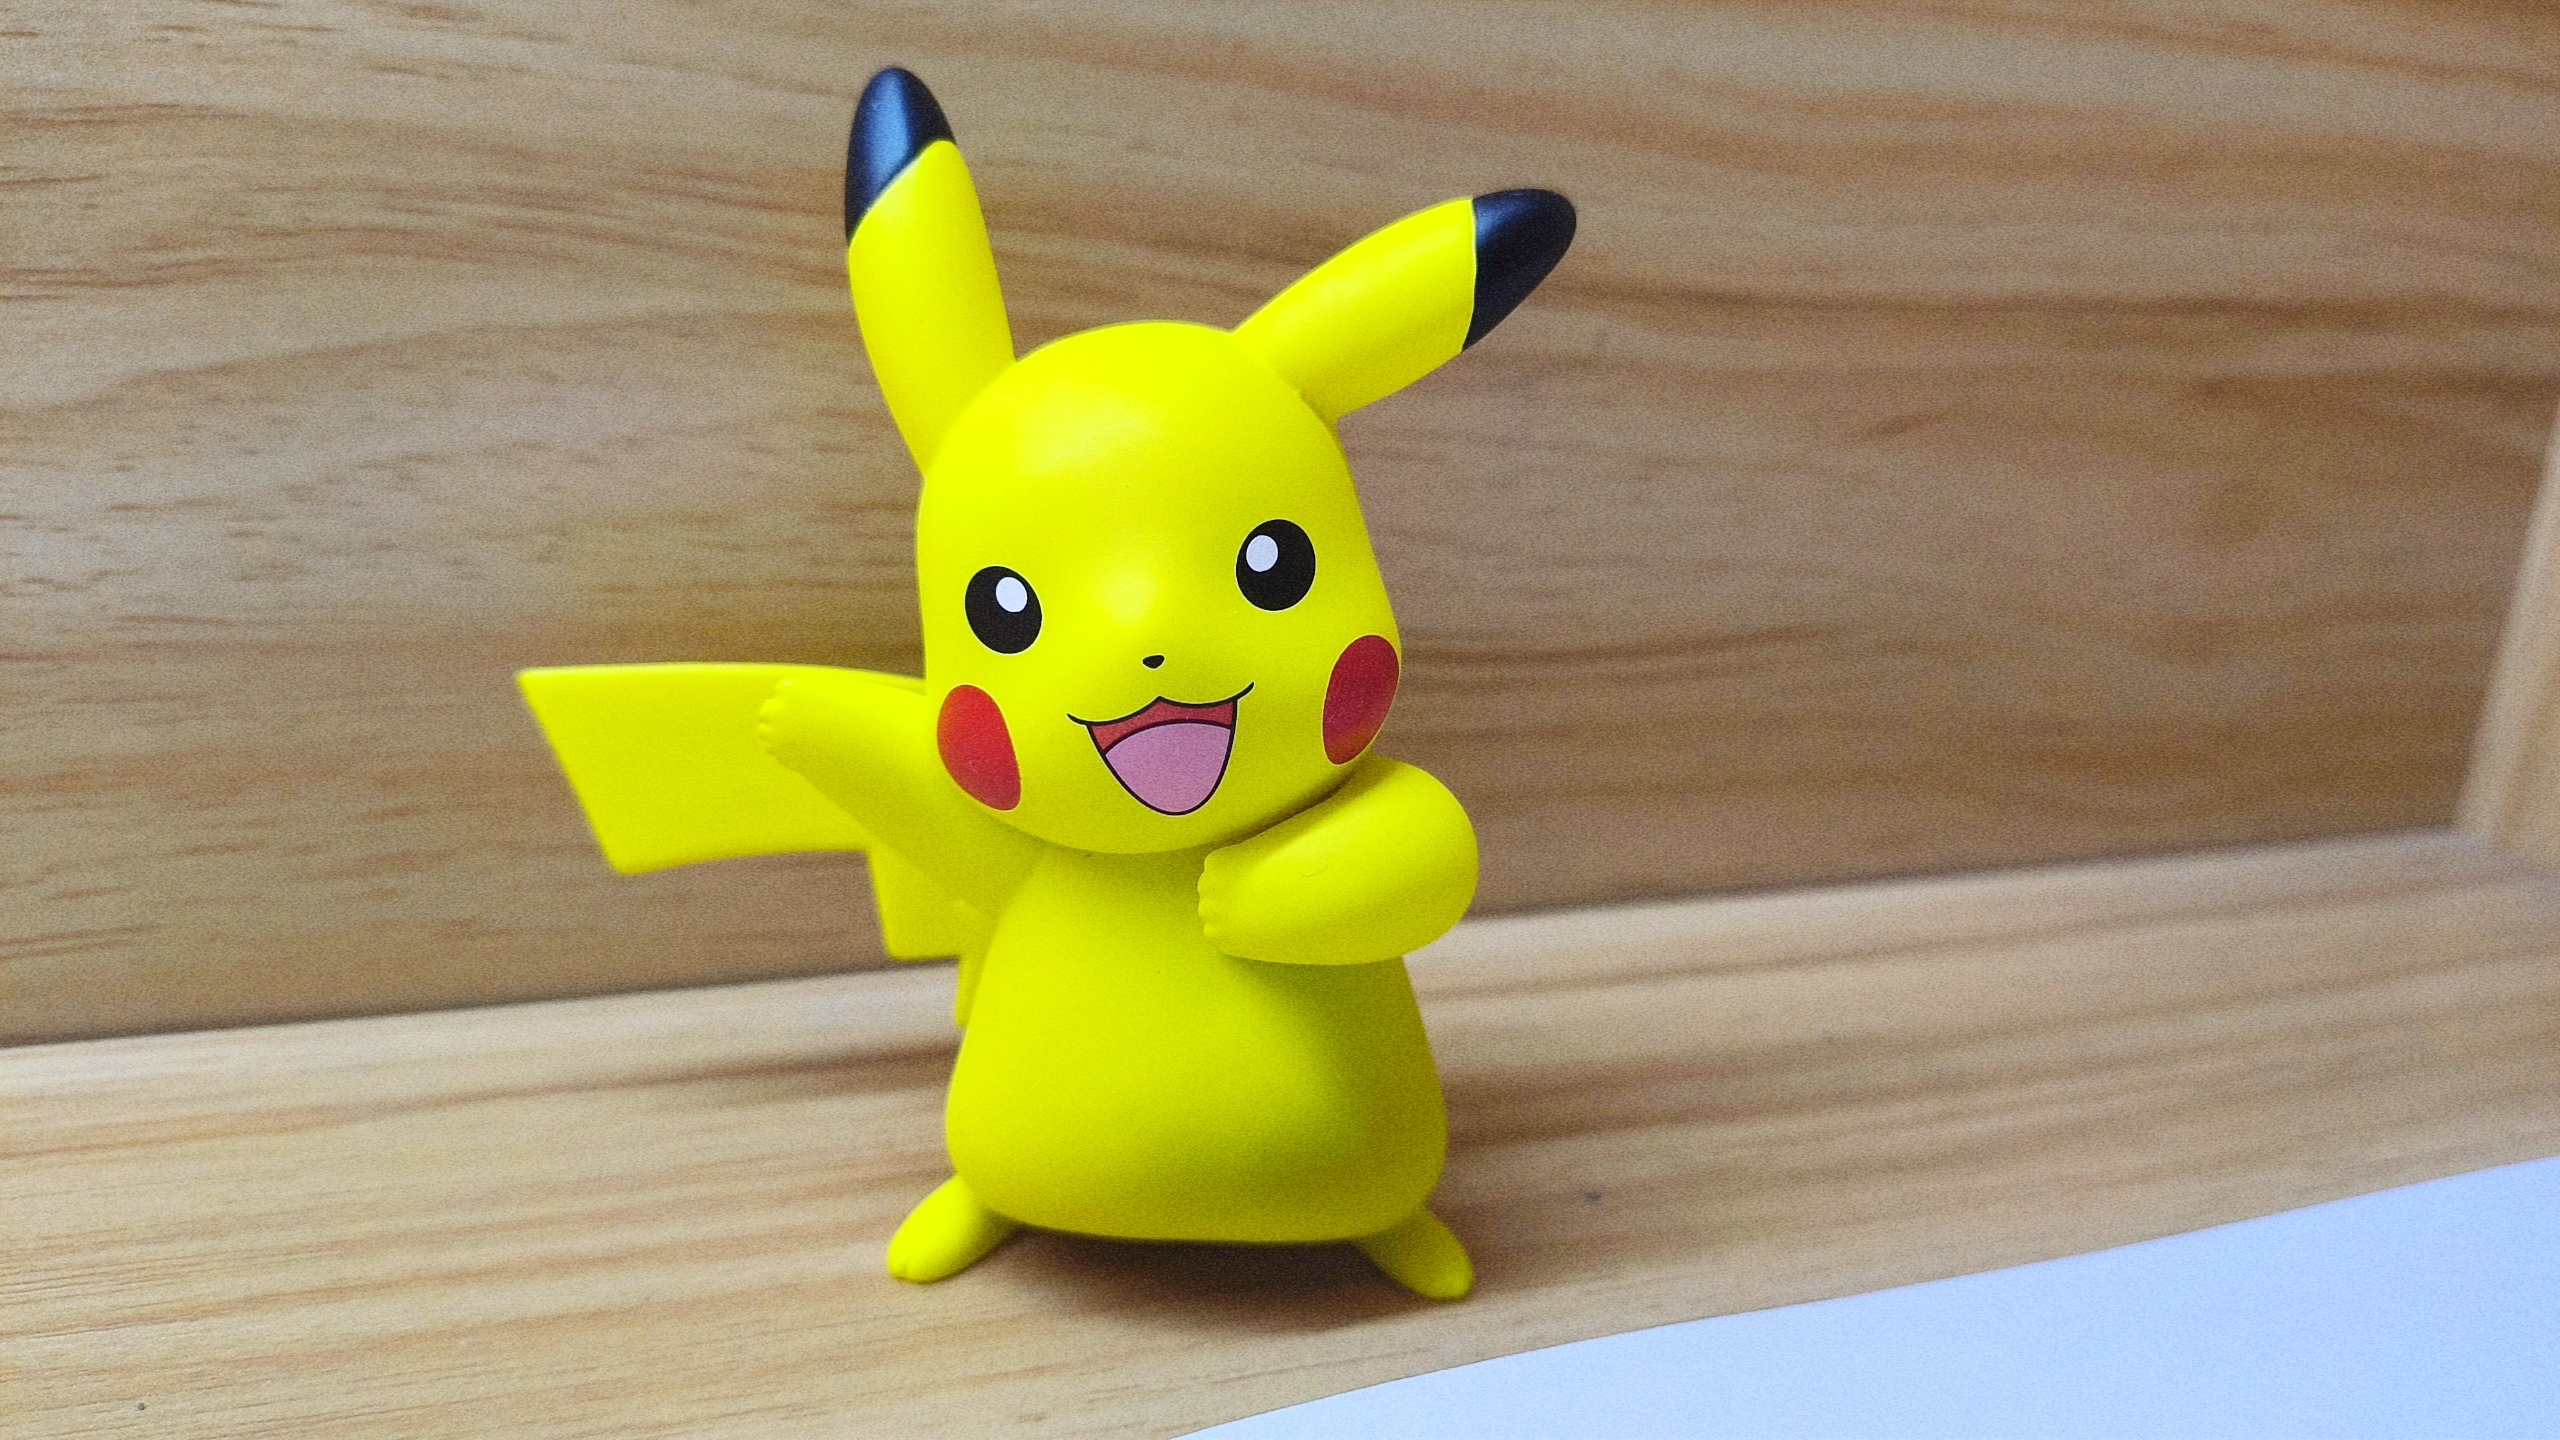
\includegraphics[scale=0.1, ]{figures/pikachu.jpg}
        \caption{这是图表}
        %\label{fig:1}
    \end{figure}

    \subsection{表格}

    \begin{table}[htbp]
        \centering
        \caption{这是表格}
        %\label{tab:1}
        \begin{tabular}{|c|c|c|}
            \hline
            \multicolumn{1}{|c|}{\textbf{表格}} & \multicolumn{1}{c|}{\textbf{表格}} & \multicolumn{1}{c|}{\textbf{表格}} \\ \hline
            \multicolumn{1}{|c|}{\textbf{表格}} & \multicolumn{1}{c|}{\textbf{表格}} & \multicolumn{1}{c|}{\textbf{表格}} \\ \hline
            \multicolumn{1}{|c|}{\textbf{表格}} & \multicolumn{1}{c|}{\textbf{表格}} & \multicolumn{1}{c|}{\textbf{表格}} \\ \hline
        \end{tabular}
    \end{table}
    \section{基础功能测试}
    \section{文字与段落}
    这是文字。

    这是段落。这是段落。这是段落。这是段落。这是段落。这是段落。这是段落。这是段落。这是段落。这是段落。这是段落。这是段落。这是段落。这是段落。这是段落。这是段落。这是段落。这是段落。
    \section{图表}

    \subsection{图片}

    \begin{figure}[htbp]
        \centering
        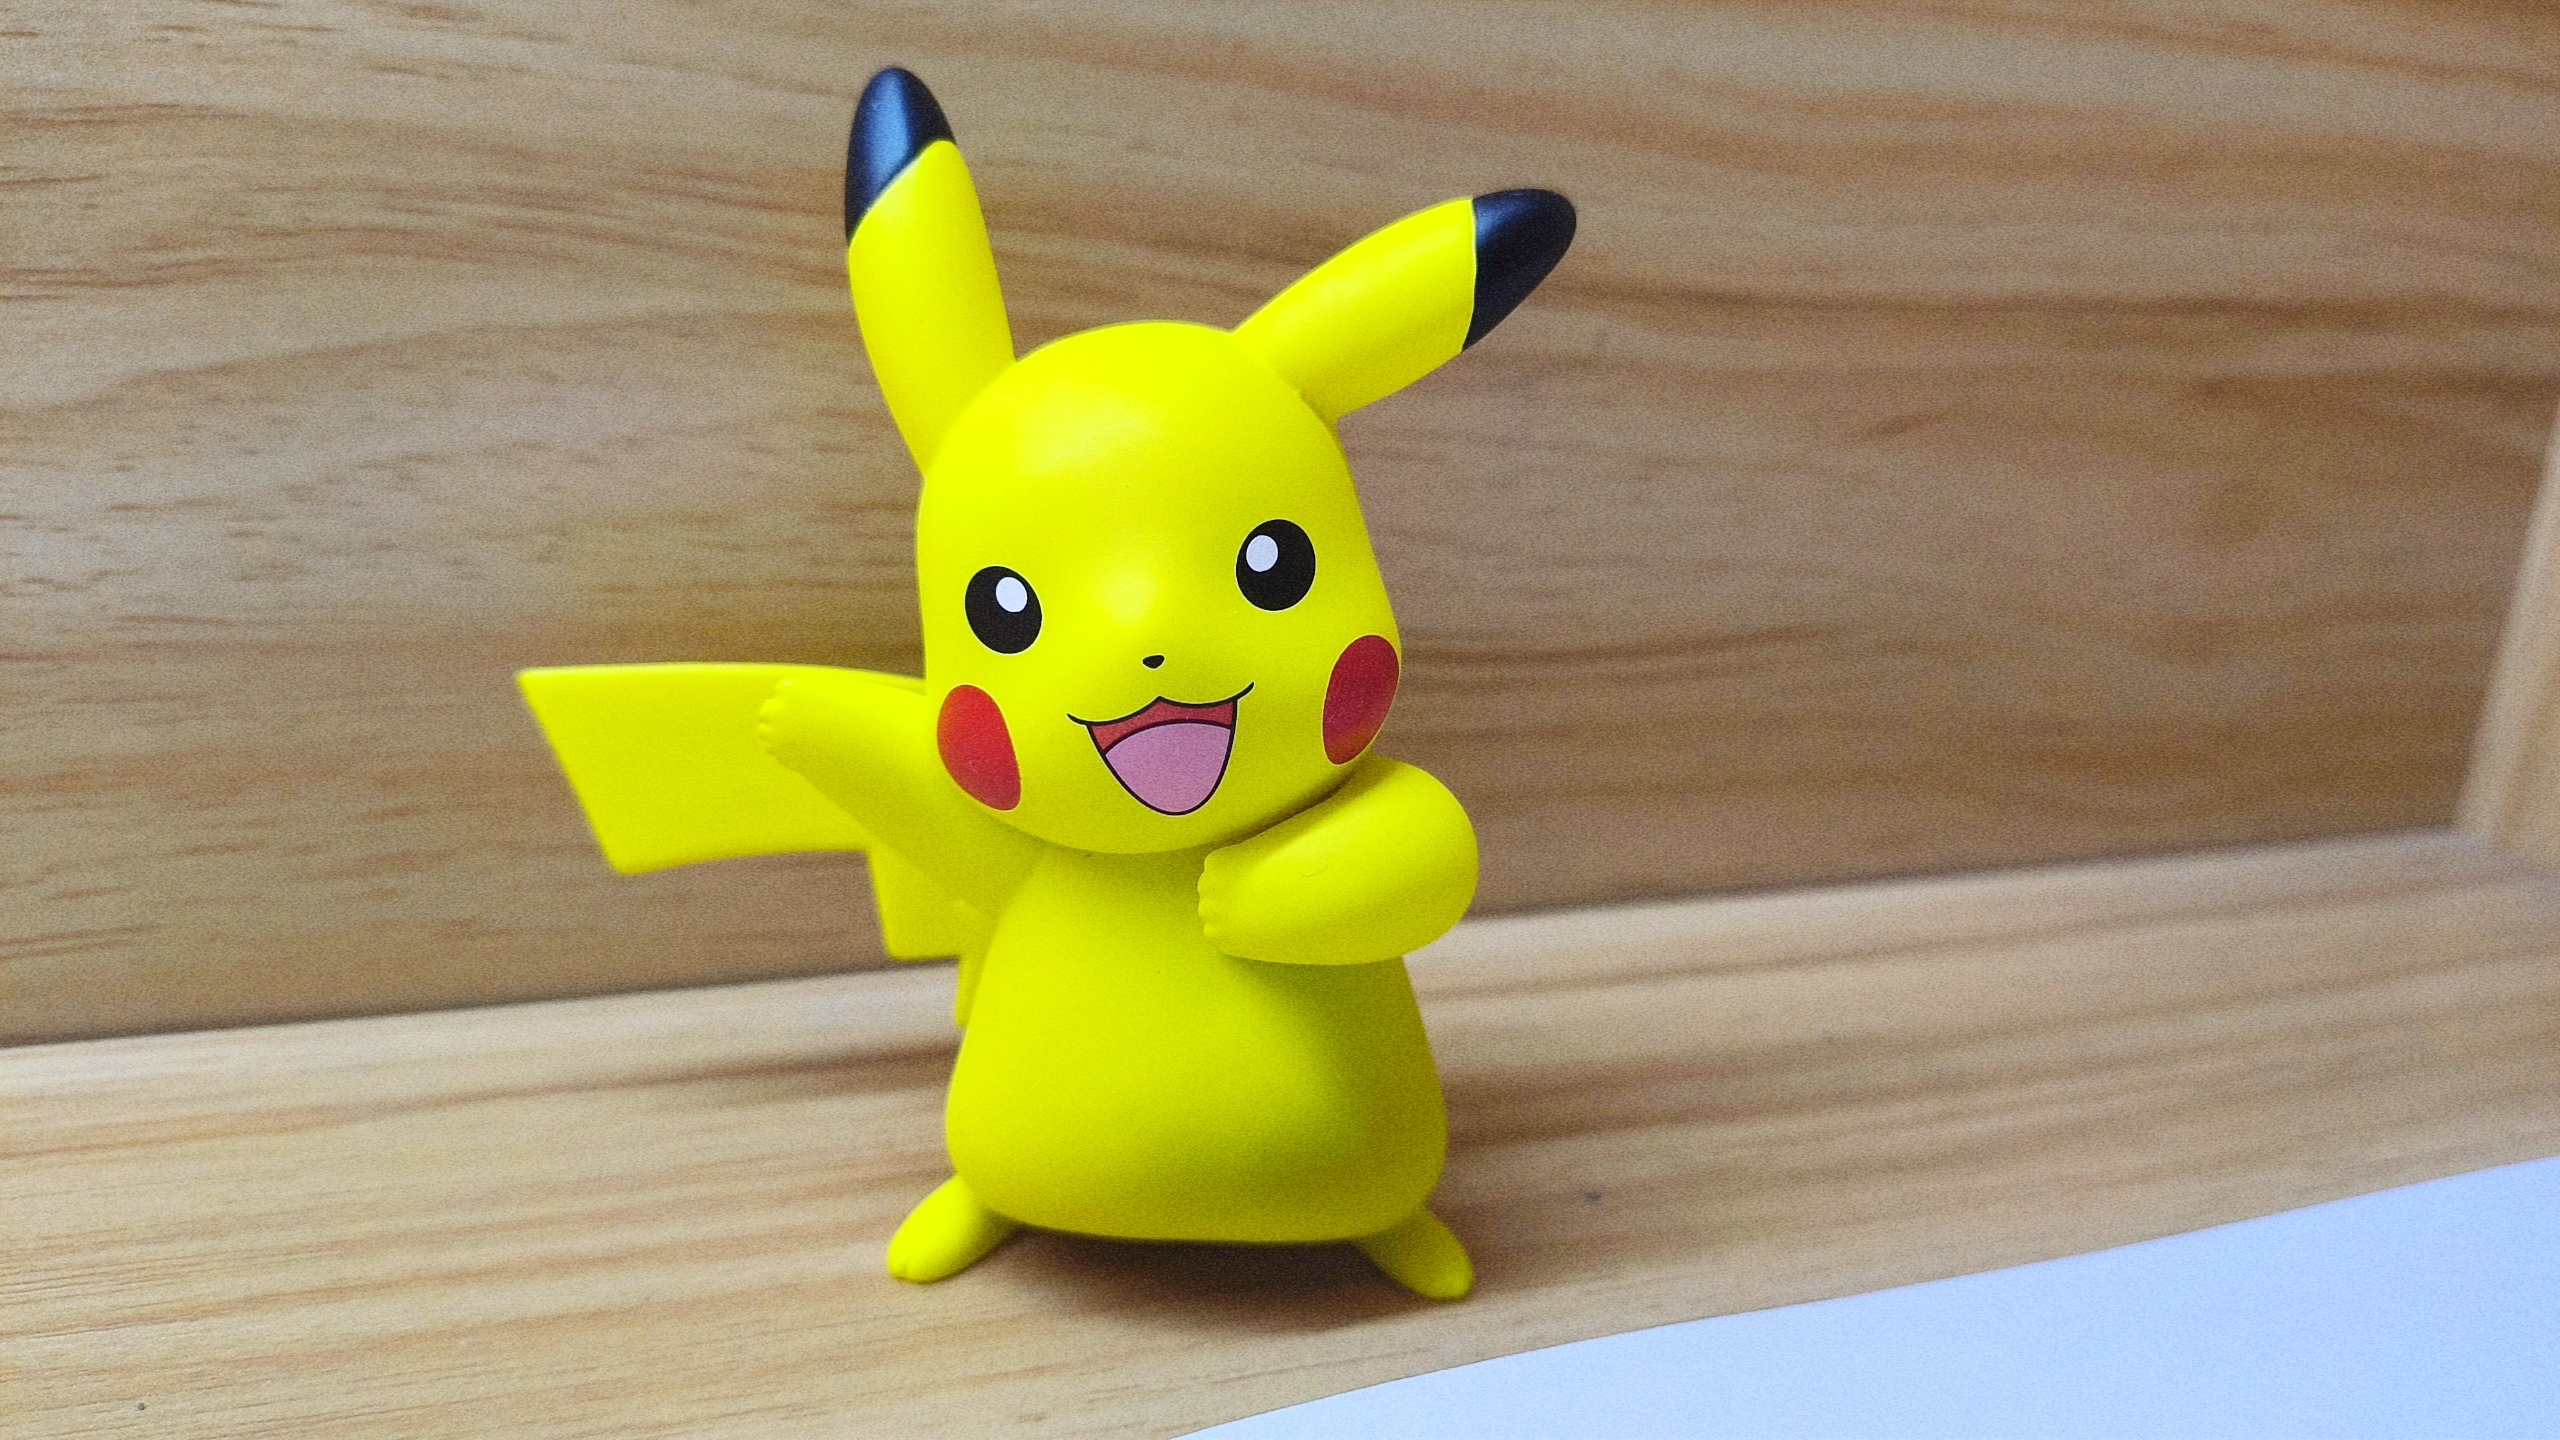
\includegraphics[scale=0.1, ]{figures/pikachu.jpg}
        \caption{这是图表}
        %\label{fig:1}
    \end{figure}

    \subsection{表格}

    \begin{table}[htbp]
        \centering
        \caption{这是表格}
        %\label{tab:1}
        \begin{tabular}{|c|c|c|}
            \hline
            \multicolumn{1}{|c|}{\textbf{表格}} & \multicolumn{1}{c|}{\textbf{表格}} & \multicolumn{1}{c|}{\textbf{表格}} \\ \hline
            \multicolumn{1}{|c|}{\textbf{表格}} & \multicolumn{1}{c|}{\textbf{表格}} & \multicolumn{1}{c|}{\textbf{表格}} \\ \hline
            \multicolumn{1}{|c|}{\textbf{表格}} & \multicolumn{1}{c|}{\textbf{表格}} & \multicolumn{1}{c|}{\textbf{表格}} \\ \hline
        \end{tabular}
    \end{table}
    \section{基础功能测试}
    \section{文字与段落}
    这是文字。

    这是段落。这是段落。这是段落。这是段落。这是段落。这是段落。这是段落。这是段落。这是段落。这是段落。这是段落。这是段落。这是段落。这是段落。这是段落。这是段落。这是段落。这是段落。
    \section{文字与段落}
    这是文字。

    这是段落。这是段落。这是段落。这是段落。这是段落。这是段落。这是段落。这是段落。这是段落。这是段落。这是段落。这是段落。这是段落。这是段落。这是段落。这是段落。这是段落。这是段落。
    \section{文字与段落}
    这是文字。

    这是段落。这是段落。这是段落。这是段落。这是段落。这是段落。这是段落。这是段落。这是段落。这是段落。这是段落。这是段落。这是段落。这是段落。这是段落。这是段落。这是段落。这是段落。
    \section{文字与段落}
    这是文字。

    这是段落。这是段落。这是段落。这是段落。这是段落。这是段落。这是段落。这是段落。这是段落。这是段落。这是段落。这是段落。这是段落。这是段落。这是段落。这是段落。这是段落。这是段落。
    \section{图表}

    \subsection{图片}

    \begin{figure}[htbp]
        \centering
        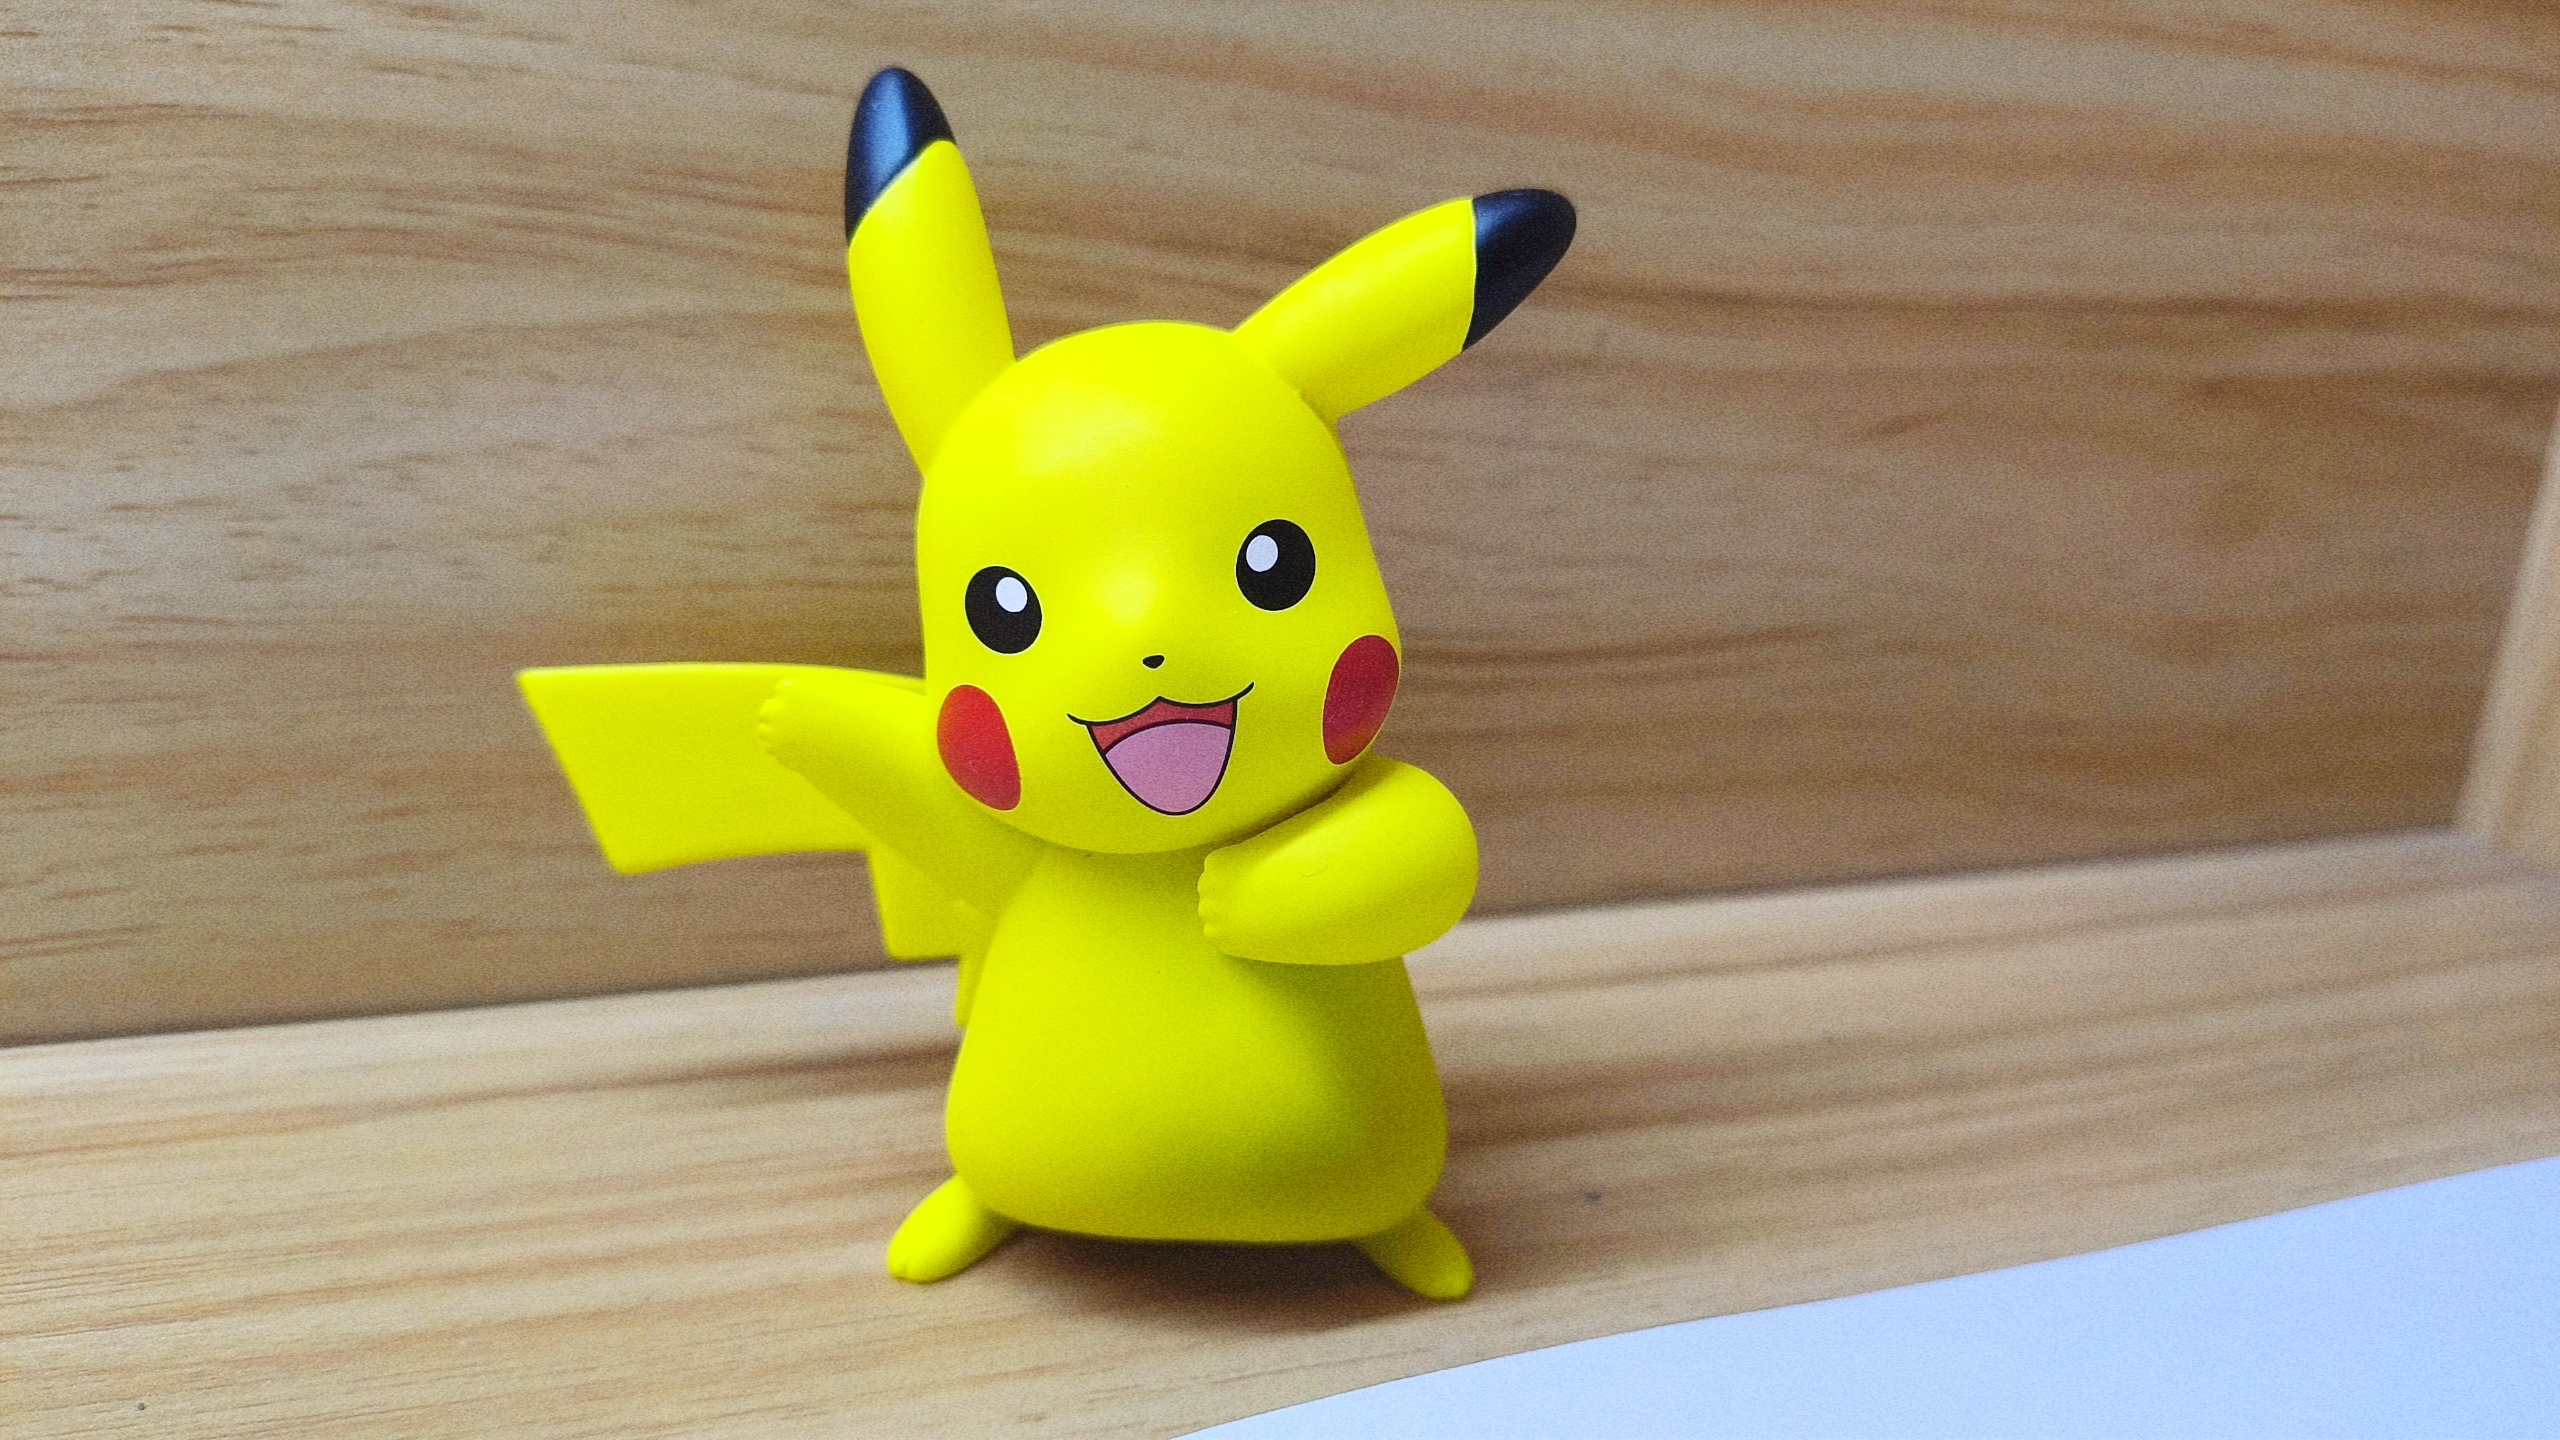
\includegraphics[scale=0.1, ]{figures/pikachu.jpg}
        \caption{这是图表}
        %\label{fig:1}
    \end{figure}

    \subsection{表格}

    \begin{table}[htbp]
        \centering
        \caption{这是表格}
        %\label{tab:1}
        \begin{tabular}{|c|c|c|}
            \hline
            \multicolumn{1}{|c|}{\textbf{表格}} & \multicolumn{1}{c|}{\textbf{表格}} & \multicolumn{1}{c|}{\textbf{表格}} \\ \hline
            \multicolumn{1}{|c|}{\textbf{表格}} & \multicolumn{1}{c|}{\textbf{表格}} & \multicolumn{1}{c|}{\textbf{表格}} \\ \hline
            \multicolumn{1}{|c|}{\textbf{表格}} & \multicolumn{1}{c|}{\textbf{表格}} & \multicolumn{1}{c|}{\textbf{表格}} \\ \hline
        \end{tabular}
    \end{table}
    \chapter{基础功能测试}
    \section{文字与段落}
    这是文字。

    这是段落。这是段落。这是段落。这是段落。这是段落。这是段落。这是段落。这是段落。这是段落。这是段落。这是段落。这是段落。这是段落。这是段落。这是段落。这是段落。这是段落。这是段落。
    \section{图表}

    \subsection{图片}

    \begin{figure}[htbp]
        \centering
        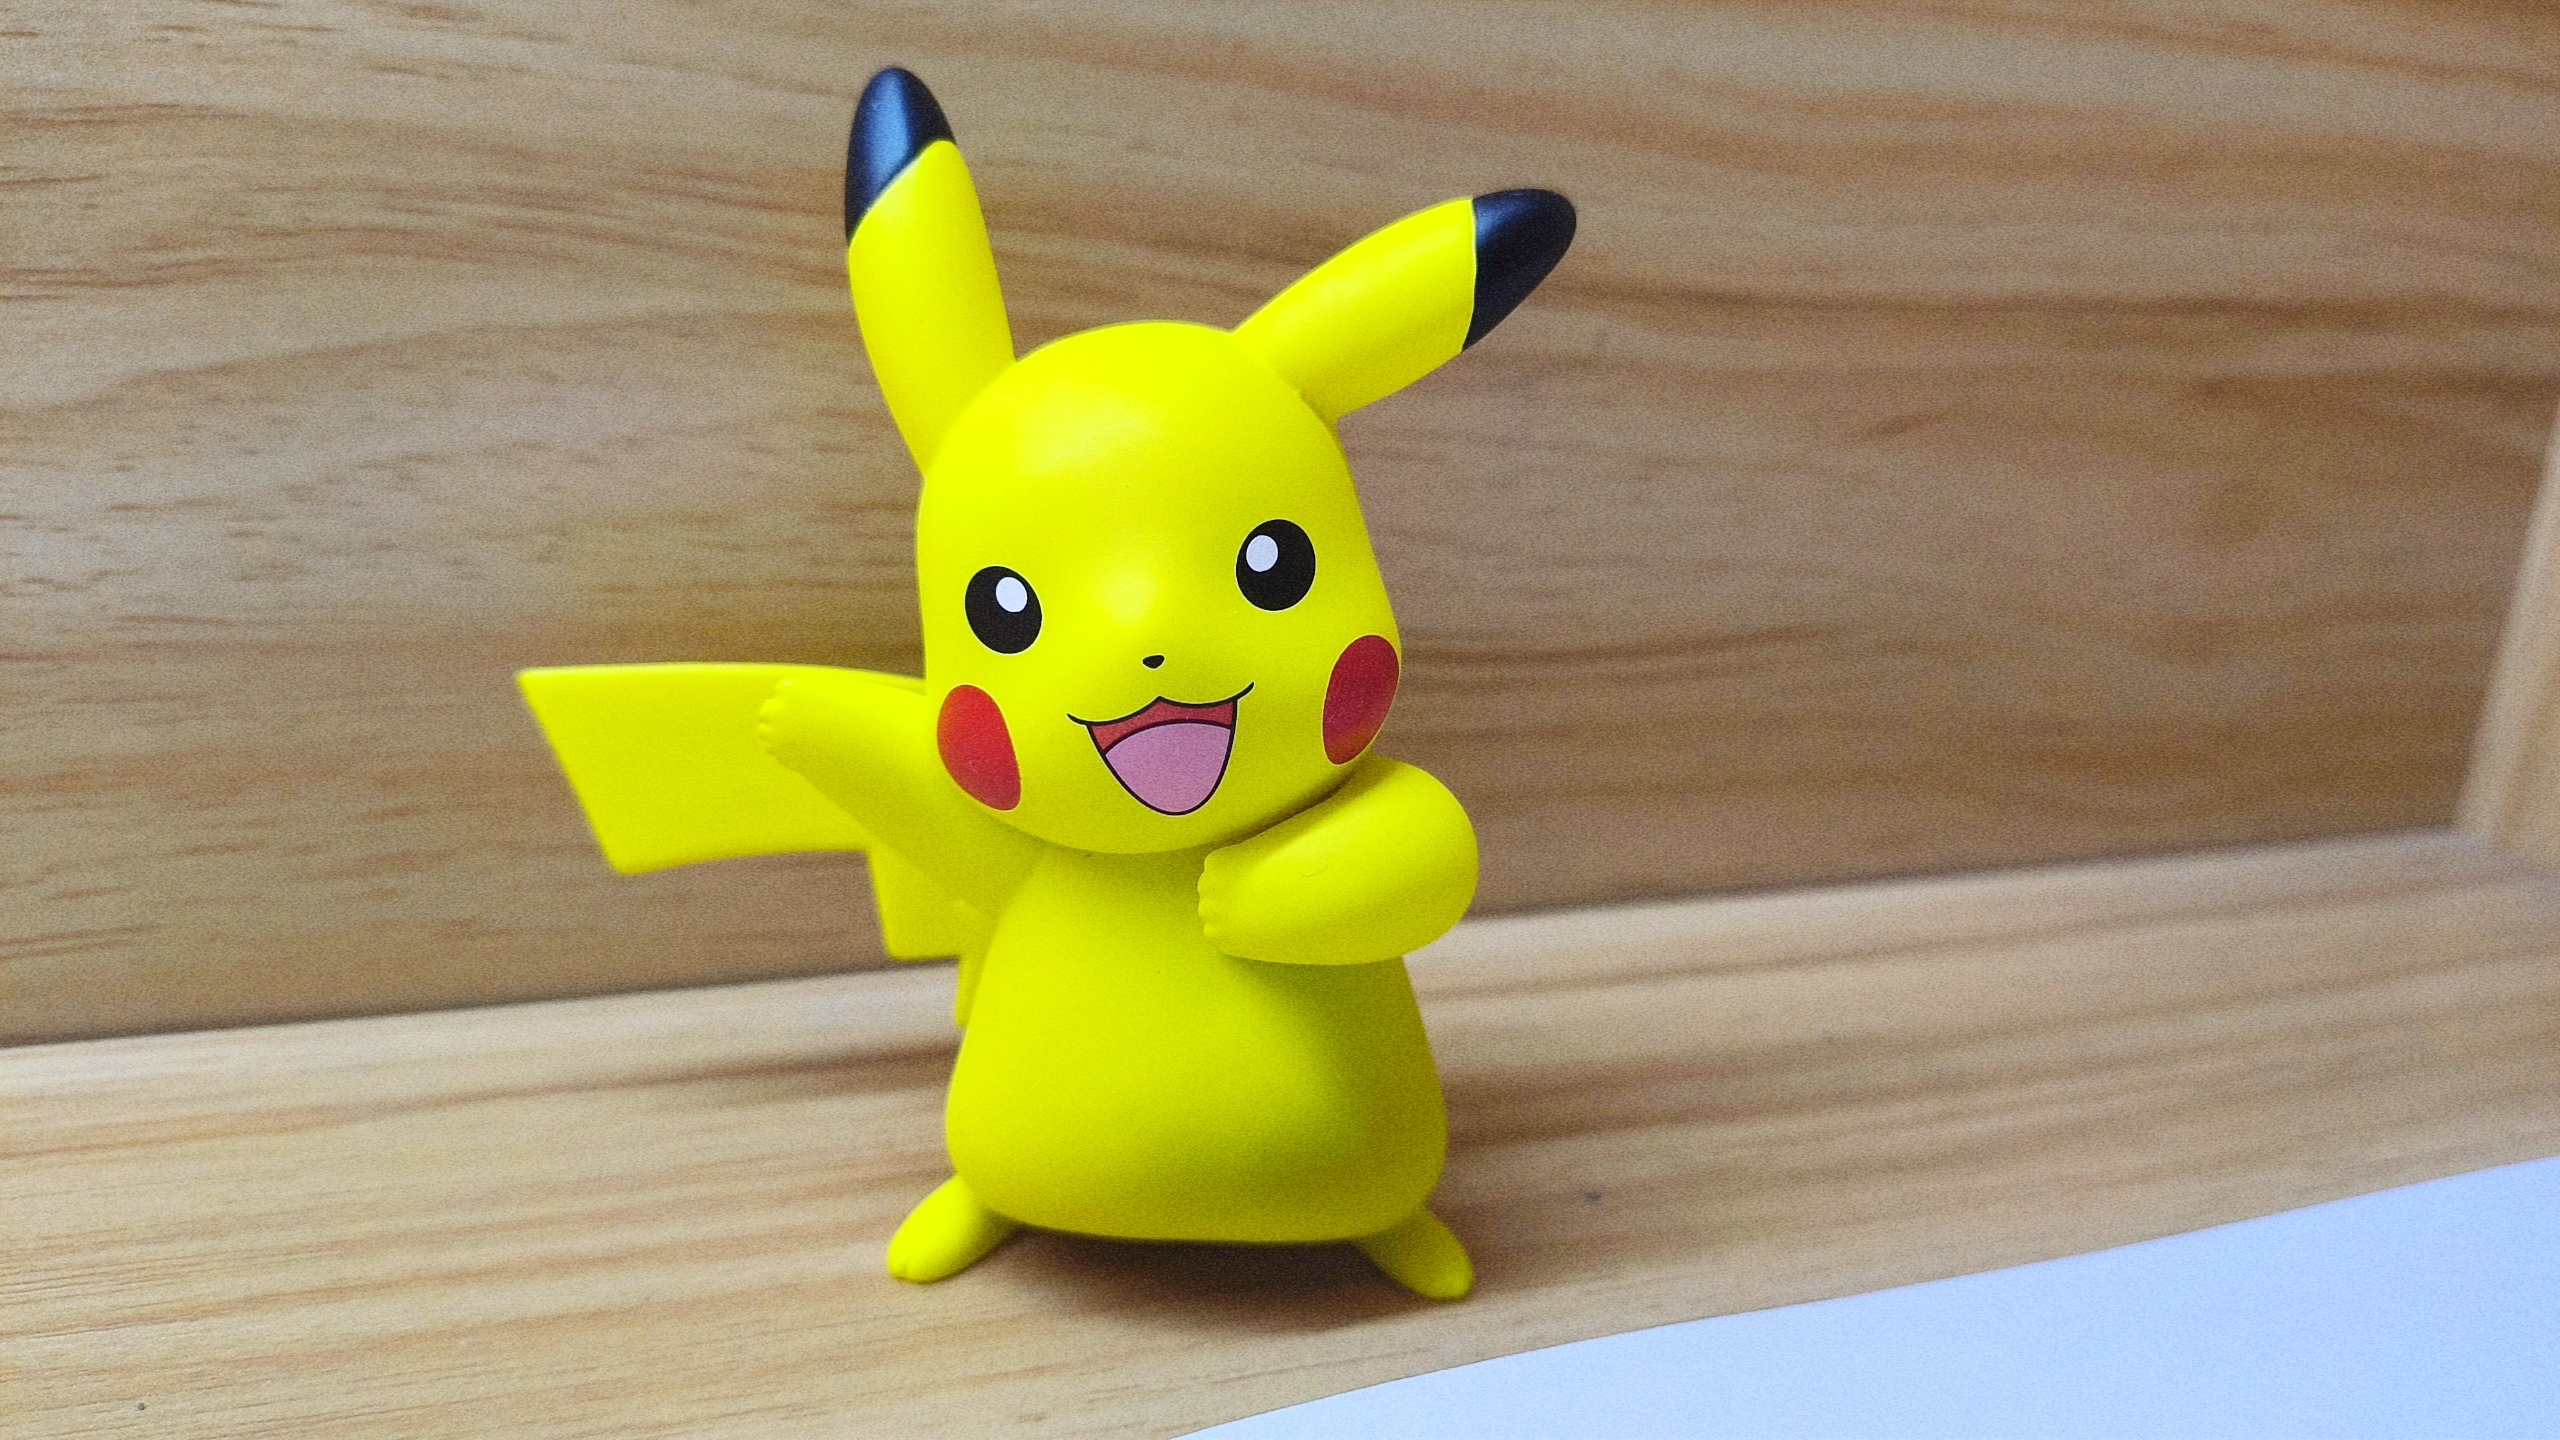
\includegraphics[scale=0.1, ]{figures/pikachu.jpg}
        \caption{这是图表}
        %\label{fig:1}
    \end{figure}

    \subsection{表格}

    \begin{table}[htbp]
        \centering
        \caption{这是表格}
        %\label{tab:1}
        \begin{tabular}{|c|c|c|}
            \hline
            \multicolumn{1}{|c|}{\textbf{表格}} & \multicolumn{1}{c|}{\textbf{表格}} & \multicolumn{1}{c|}{\textbf{表格}} \\ \hline
            \multicolumn{1}{|c|}{\textbf{表格}} & \multicolumn{1}{c|}{\textbf{表格}} & \multicolumn{1}{c|}{\textbf{表格}} \\ \hline
            \multicolumn{1}{|c|}{\textbf{表格}} & \multicolumn{1}{c|}{\textbf{表格}} & \multicolumn{1}{c|}{\textbf{表格}} \\ \hline
        \end{tabular}
    \end{table}
\end{ujnbody}